\documentclass[11pt,letterpaper]{article}

% Load some basic packages that are useful to have
% and that should be part of any LaTeX installation.
%
% be able to include figures
\usepackage{graphicx}
% get nice colors
\usepackage{xcolor}

% change default font to Palatino (looks nicer!)
\usepackage[latin1]{inputenc}
\usepackage{mathpazo}
\usepackage[T1]{fontenc}
% load some useful math symbols/fonts
\usepackage{latexsym,amsfonts,amsmath,amssymb}

% comfort package to easily set margins
\usepackage[top=1in, bottom=1in, left=1in, right=1in]{geometry}
\usepackage{hyperref}
\usepackage[all]{hypcap}
% control some spacings
%
% spacing after a paragraph\begin{figure}[bth]
\setlength{\parskip}{.15cm}
% indentation at the top of a new paragraph
\setlength{\parindent}{0.0cm}

\begin{document}

\begin{center}
\Large
Ay190 -- Worksheet 16\\
David Vartanyan\\
Date: \today
\end{center}

\section{}

The code uses the mydata class of objects to store and easily access variables.
We devise a grid over an x-domain and apply initial data. We reconstruct the primitives at cell interfaces and use our EOS to find pressure using a variety of different order methods (i.e. PC, TVD-minmod, TVD-MC2). We integrate forward in time using RK2 and find fluxes using Euler's equations.

See Figures ~\ref{fig:1}, ~\ref{fig:2}, ~\ref{fig:3}, ~\ref{fig:4} for time evolution using the PC reconstruction.

See Figures ~\ref{fig:5} and ~\ref{fig:6} for the minmod and pc reconstructoins at $0.399$s. All Figures include density, velocity, and pressure evolutions. The x-axes is the spatial domain.

We see the development and spilling over of a density divide on the shock front.
The plots exhibit similar behavior to the exact solution from ws15.

\begin{figure}[bth]
\centering
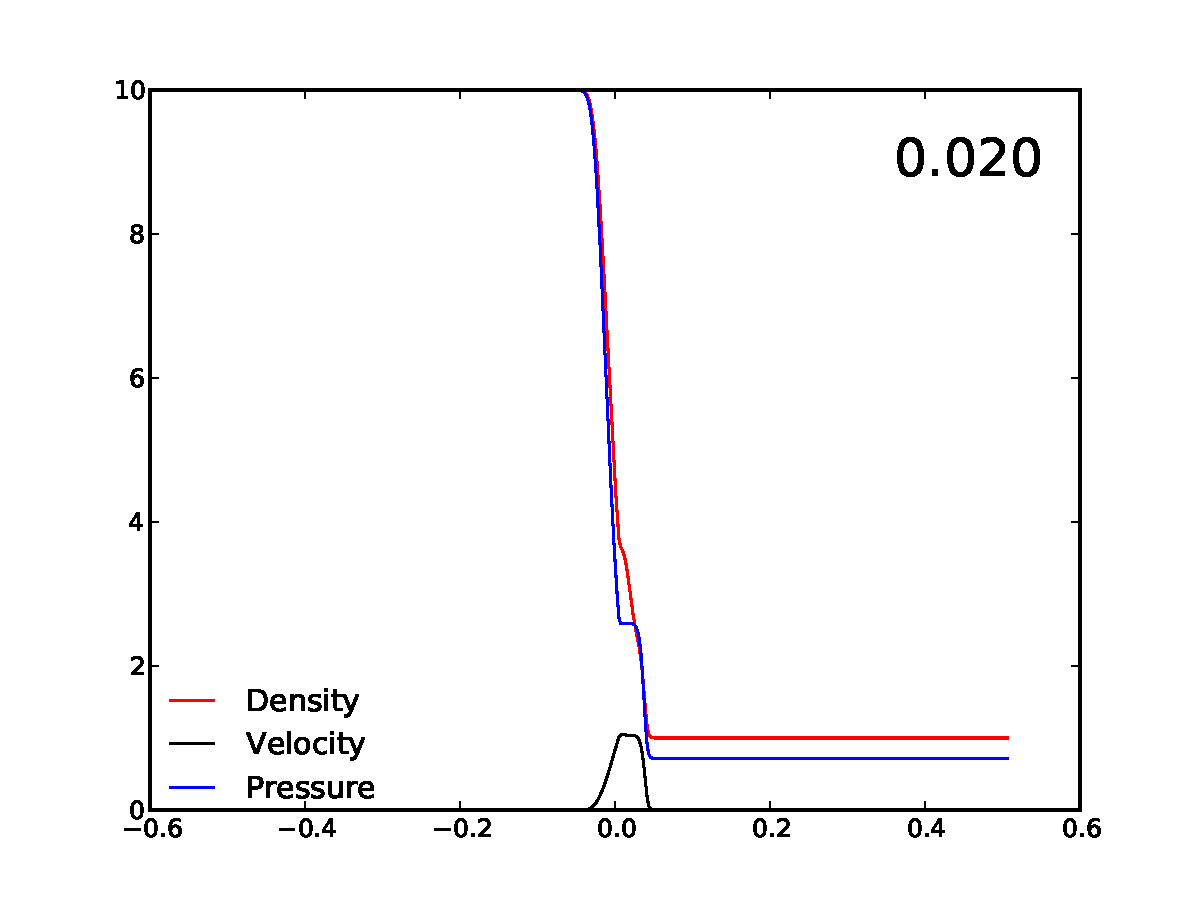
\includegraphics[width=0.7\textwidth]{t100.pdf}
\caption{Shocks $0.02$ seconds in}
\label{fig:1}
\end{figure}

\begin{figure}[bth]
\centering
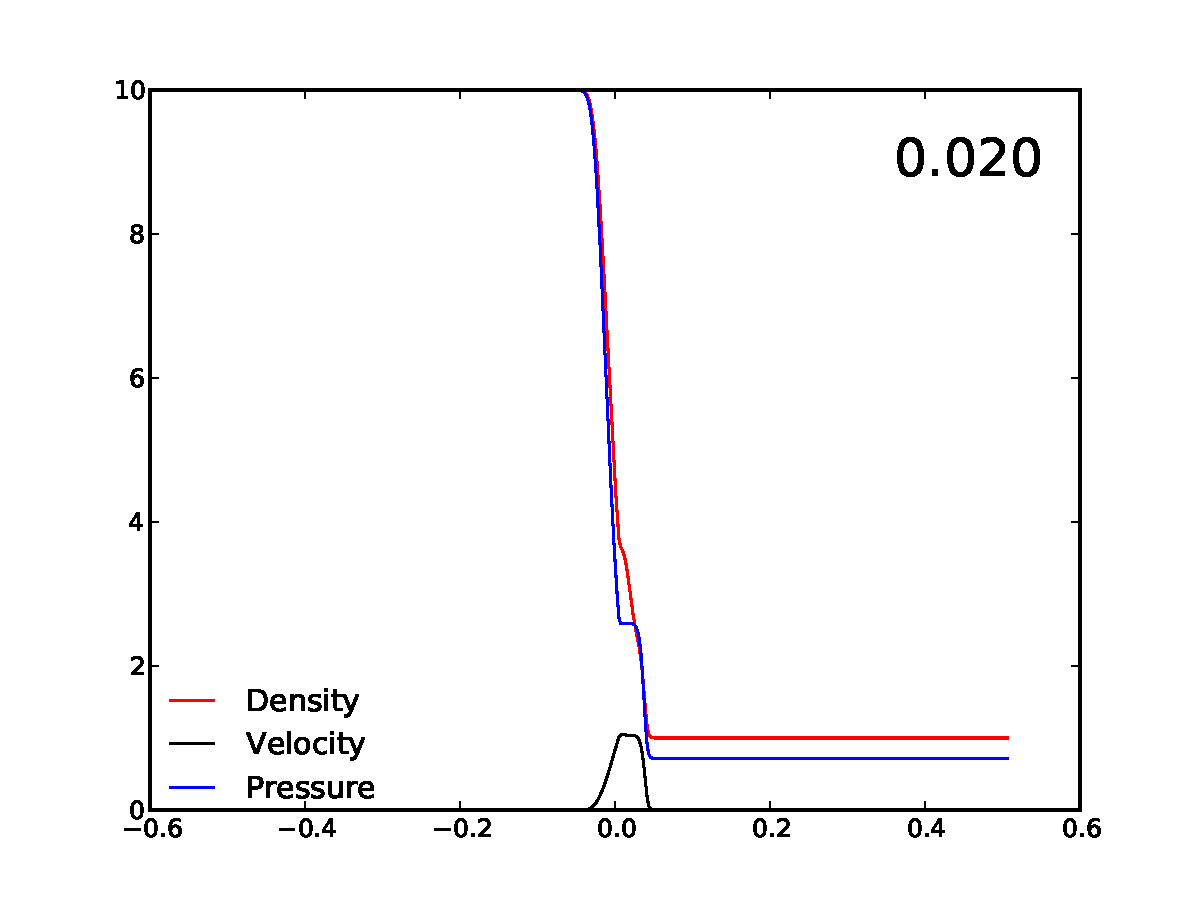
\includegraphics[width=0.7\textwidth]{t100.pdf}
\caption{Shocks $0.065$ seconds in}
\label{fig:2}
\end{figure}

\begin{figure}[bth]
\centering
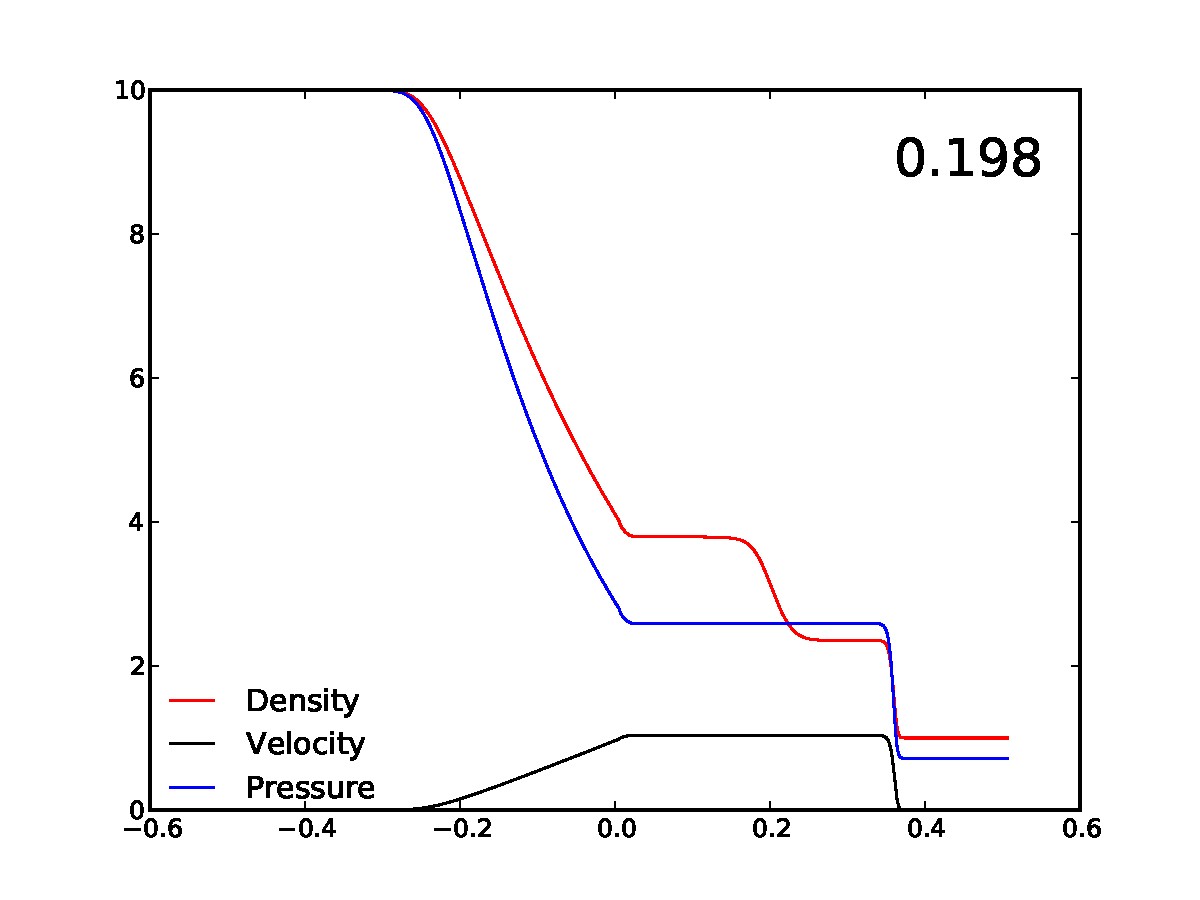
\includegraphics[width=0.7\textwidth]{t500.pdf}
\caption{Shocks $0.195$ seconds in}
\label{fig:3}
\end{figure}

\begin{figure}[bth]
\centering
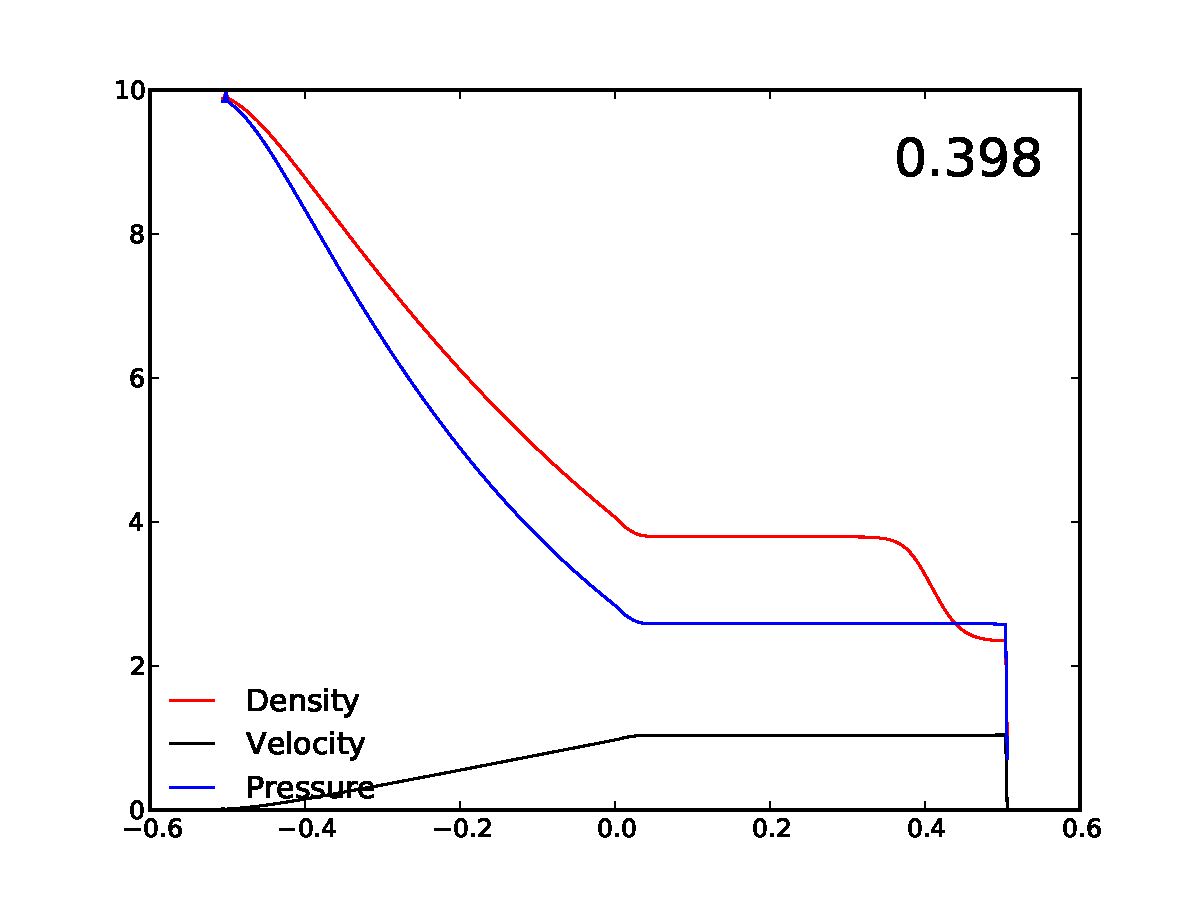
\includegraphics[width=0.7\textwidth]{t950.pdf}
\caption{Shocks $0.398$ seconds in}
\label{fig:4}
\end{figure}

\begin{figure}[bth]
\centering
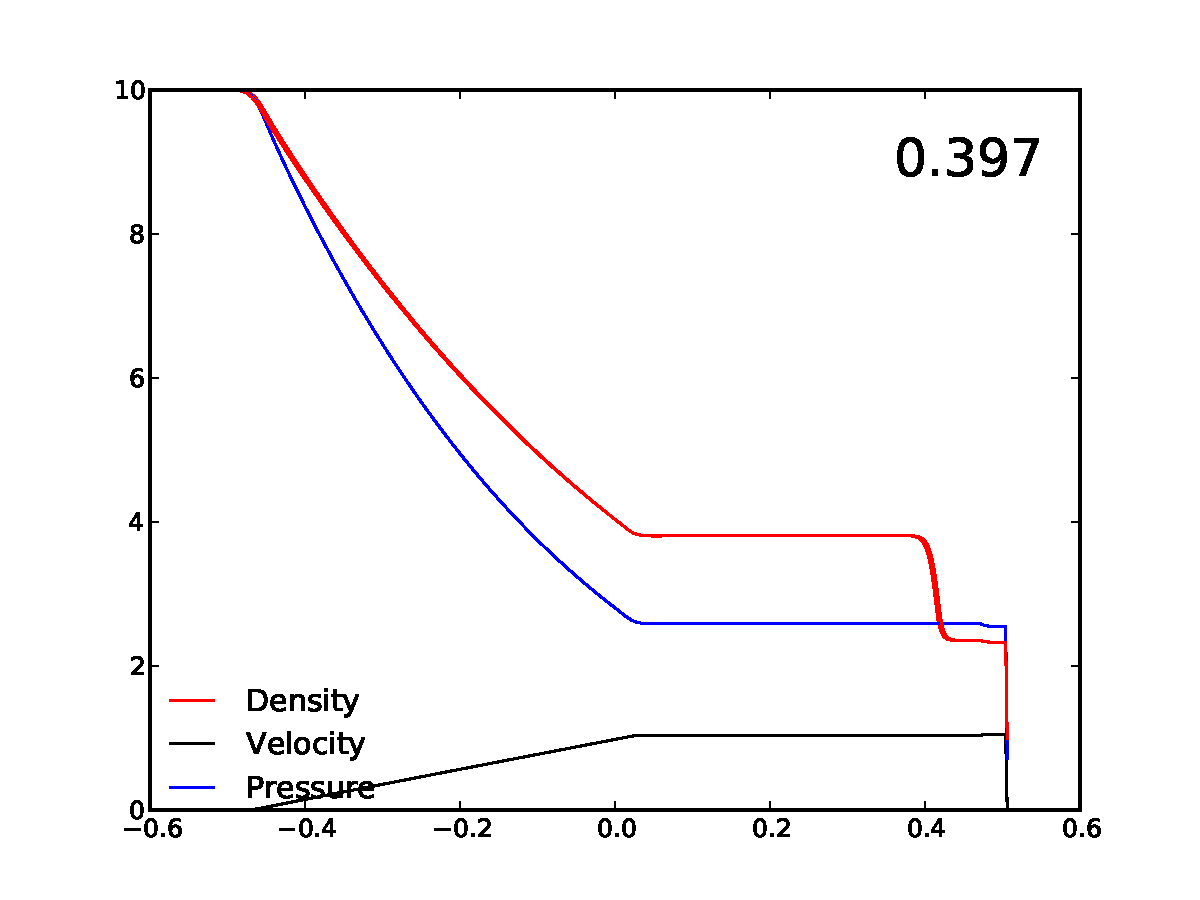
\includegraphics[width=0.7\textwidth]{minmod.pdf}
\caption{minmod 0.399s in}
\label{fig:5}
\end{figure}



\begin{figure}[bth]
\centering
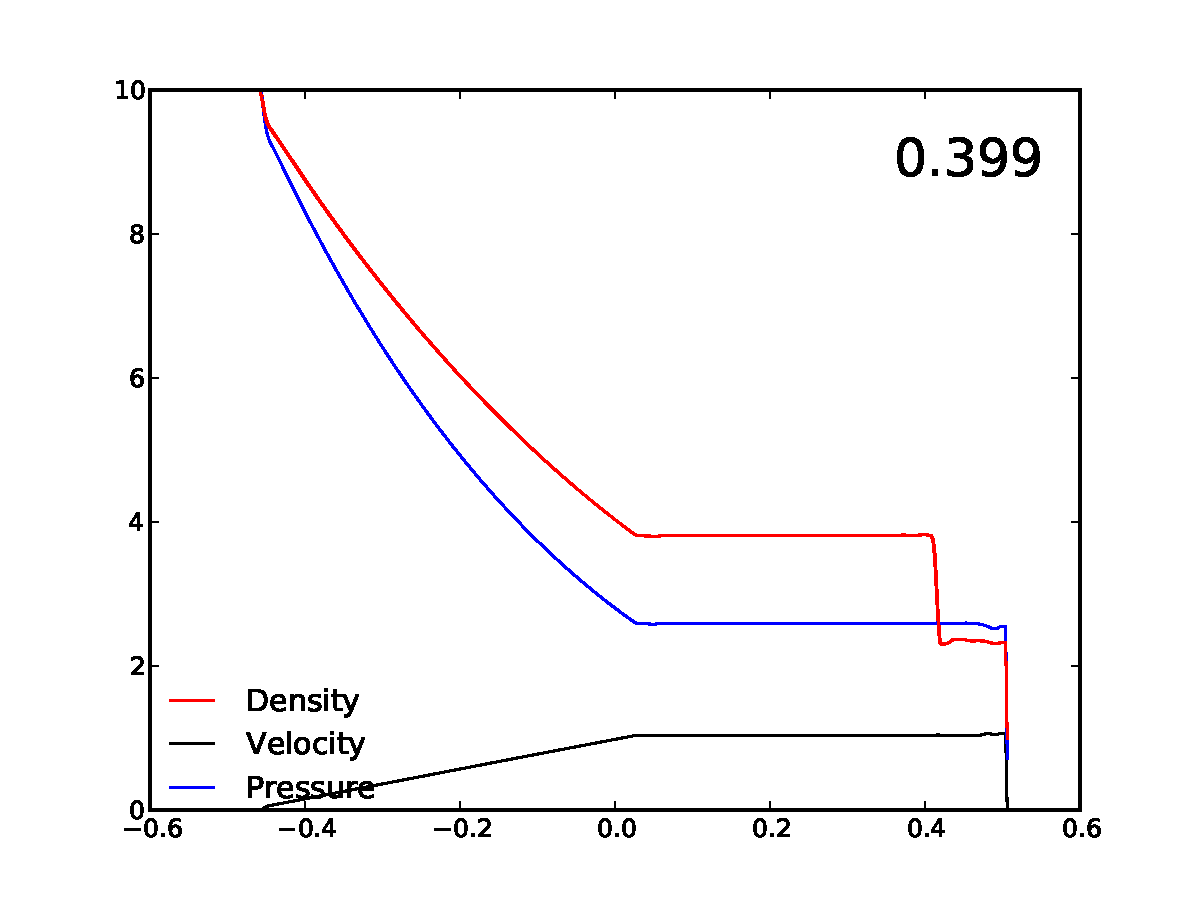
\includegraphics[width=0.7\textwidth]{mc.pdf}
\caption{mc $0.399$ seconds in}
\label{fig:6}
\end{figure}


\end{document}

